\documentclass[a4paper,8pt]{article} % Prepara un documento per carta A4, con un font di dimensione 12pt

\usepackage[italian]{babel} % Adatta LaTeX alle convenzioni tipografiche italiane,
% e ridefinisce alcuni titoli in italiano, come "Capitolo" al posto di "Chapter",
% se il vostro documento è in italiano
% l'opzione  linguistica 'french' è necessaria per l'abilitazione della
% successiva istruzione <<\frenchspacing>> 
\usepackage[T1]{fontenc} % Riga da togliere se si compila con PDFLaTeX
\usepackage[utf8]{inputenc} % Consente l'uso caratteri accentati italiani
\usepackage{amsthm}
\usepackage[margin=1.1in]{geometry}
\usepackage{hyperref}
\usepackage{ragged2e}
\RaggedRight

\usepackage{listings}
\usepackage{xcolor}
\usepackage{enumitem}
\usepackage{hyperref}

\usepackage{graphicx}
\graphicspath{ {./images/} }


\setlist[enumerate]{label*=\arabic*.}

\definecolor{codegreen}{rgb}{0,0.6,0}
\definecolor{codegray}{rgb}{0.5,0.5,0.5}
\definecolor{codepurple}{rgb}{0.58,0,0.82}
\definecolor{backcolour}{rgb}{0.95,0.95,0.92}

\lstdefinestyle{mystyle}{
    backgroundcolor=\color{backcolour},   
    commentstyle=\color{codegreen},
    keywordstyle=\color{magenta},
    numberstyle=\tiny\color{codegray},
    stringstyle=\color{codepurple},
    basicstyle=\ttfamily\footnotesize,
    breakatwhitespace=false,         
    breaklines=true,                 
    captionpos=b,                    
    keepspaces=true,                 
    numbers=left,                    
    numbersep=5pt,                  
    showspaces=false,                
    showstringspaces=false,
    showtabs=false,                  
    tabsize=2,
}


\lstset{style=mystyle}

\def\code#1{\texttt{#1}}
\title{Winsome --- progetto di laboratorio di reti} % \LaTeX è una macro che compone il logo "LaTeX"
% I commenti (introdotti da %) vengono ignorati

\author{Samuele Bonini}
\date{10 gennaio 2022}
% in alternativa a \date il comando \today introduce la data di sistema.
\begin{document}


\maketitle % Genera il titolo sulle istruzioni  \title, \author e \date



\tableofcontents % Prepara l'indice generale
\setlength{\parskip}{0.5em}

\section{Note sulla compilazione ed esecuzione}
Per compilare il progetto, \textbf{si esegua lo script} \code{compile.sh}, collocato all'interno della root del progetto.
Lo script reperisce i file \code{.java}  necessari alla compilazione dalle \emph{classh paths} e utilizza il comando \code{javac} per creare la build,
includendo anche i file \code{.jar} delle librerie esterne utilizzate (\href{https://twin.sh/articles/8/how-to-compile-large-java-projects-from-terminal}{fonte}).

\par Per eseguire la classe \code{MainClient}, si esegua lo script \code{client.sh}, mentre per la classe \code{MainServer} (che deve essere
eseguita prima del client), si esegua lo script \code{server.sh}. Entrambe le classi possono altresì essere utilizzate via i rispettivi file \code{jar}, entrambi collocati nella root directory.

\section{Architettura di massima del progetto} %
\subsection{Suddivisione in layer}
Nella realizzazione del software in oggetto, si è scelto di utilizzare un'architettura a strati, suddividendo le classi in gioco
all'interno di insiemi disgiunti in base alle responsabilità e alle dipendenze. Lo scopo di utilizzare layer ben distinti è quello
di ottenere un basso grado di accoppiamento tra le componenti del sistema, mantenendo altresì una buona  \emph{separation of concerns}.
Avere un basso grado di accoppiamento tra le classi implica la possibilità di sviluppare in maniera quanto più indipendente
le varie componenti, modificandole (o anche riscrivendole da zero) all'occorrenza, oltre che avere un vantaggio nelle fasi di testing e debugging, ove è
più facile isolare eventuali fault.
\par
In seguito all'analisi dei requisiti, in fase di progettazione sono stati individuati i seguenti layer:
\begin{itemize}
    \item \textbf{Entità}: sono le classi che rappresentano il dominio dell'applicazione e incarnano l'universo delineato dal progetto
    \item \textbf{Data store}: espone le entità al mondo esterno attraverso un'interfaccia controllata e definisce le operazioni primitive sulle stesse
    \item \textbf{Business logic}: implementa operazioni più complesse servendosi dalle primitive esposte dallo store e, talvolta, dalle entità stesse;
          aggiunge controlli di vario tipo (permessi, \emph{well-formedness} delle richieste, ecc.); fornisce all'esterno un'\textsc{api} più ricca per interagire con le entità
    \item \textbf{Server}: gestisce la connessione logica coi client, espone un'\textsc{api} per accedere ai layer sottostanti secondo le regole di business, si occupa della
          formattazione e presentazione dei dati in entrata e in uscita
\end{itemize}
La regola generale è che le classi di un layer hanno dipendenze solo da classi dello stesso layer o di layer più interni (\emph{inward dependency principle}).
Si noti infine che i nomi dei layer sopracitati non sono in corrispondenza biunivoca coi package Java utilizzati nel progetto, i quali sono stati
identificati con un criterio differente e più legato ai dettagli implementativi.
\par
Il seguente diagramma delle dipendenze esemplifica il principio di \emph{inward dependency} applicato alle classi di questo progetto. Si noti che le dipendenze sono indotte solo tra classi appartenenti allo stesso
layer o verso classi dei layer più interni.

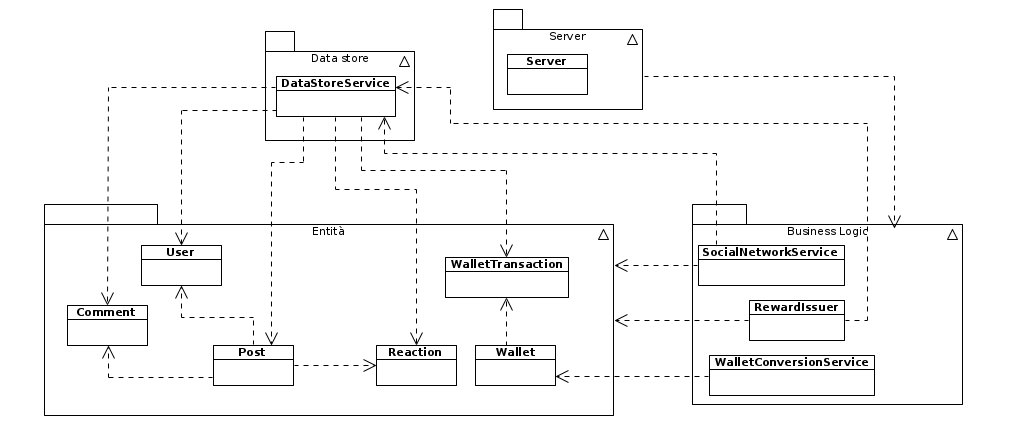
\includegraphics[width=\textwidth]{dependencies.png}

\par Questo documento è strutturato in maniera tale da illustrare, come prima cosa, le caratteristiche delle entità
di dominio e le operazioni primitive a esse associate, per poi spostarsi progressivamente sui layer
più esterni dell'architettura, dando un'idea di come le classi appartenenti allo strato della business logic sono
implementate, chiarendo infine come viene realizzata, agli atti, la comunicazione tra il server e il client.\\
\subsection{Protocollo applicazione}
Il protocollo utilizzato a livello applicativo è \textsc{http}. Il server espone un'\textsc{api} di tipo \textsc{rest} misto a \textsc{rpc}. Le richieste e le risposte \textsc{http} vengono
incarnate rispettivamente dalle classi \code{RestRequest} e \code{RestResponse}, che dispongono di metodi per convertirle da (risp. in) stringhe, consentendone
la (de)serializzazione e lettura (risp. scrittura) mediante socket.
\par L'autenticazione utilizza il protocollo \textbf{bearer token}, schema definito nell'\href{https://datatracker.ietf.org/doc/html/rfc6750}{\textsc{rfc} 6750}.
Il protcollo prevede che le richieste vengano autenticate inserendo uno header (\code{Authorization}) contenente un token di 128 bit.
La classe \code{AuthenticationMiddleware} (illustrata più in dettaglio nel seguito), responsabile della verifica delle credenziali nelle richieste \textsc{http},
controlla la presenza e la validità di questo header.
\par Il token viene ottenuto per la prima volta dal client in fase di login: la password fornita dall'utente all'atto della registrazione, che viene mantenuta
nel database criptata utilizzando l'algoritmo \href{https://en.wikipedia.org/wiki/MD5}{\textsc{md5}}, viene confrontata con quella inviata durante il login (dopo aver
cifrato anch'essa); in caso di esito positivo, il server emette un token che l'utente utilizzerà nelle successive richieste (fino al logout).


\section{Le entità di dominio}
\subsection{Gli utenti}
La classe \code{User} rappresenta un utente registrato a Winsome. A esso è associato uno username, una password (criptata come descritto nel capitolo precedente) e un \code{Set} di tag,
rappresentati da stringhe \emph{lowercase}. L'univocità dello username non è gestita a livello entità ma nello store.
\subsection{Post, commenti, reazioni}
La classe \code{Post} rappresenta un post all'interno di Winsome. Contiene informazioni circa il titolo, il contenuto e il timestamp di creazione. L'identificativo del post è uno \textsc{uuid}.
\par Il post contiene una stringa che si riferisce allo username del suo autore. La scelta di utilizzare una stringa anziché un riferimento a un oggetto \code{User} deriva dalla volontà
di gestire l'integrità referenziale a livello dello store anziché all'interno delle entità stesse: si è scelto, in altre parole, di non utilizzare l'\textbf{active record pattern}, in favore
della presenza di un layer dedicato all'accesso ai dati.
\par I commenti e le reazioni (upvote o downvote) ai post vengono aggregati all'interno di due insiemi presenti nella classe. La scelta di utilizzare un \code{TreeSet} per entrambi deriva
dalla necessità di mantenere l'ordine temporale di inserimento.
\par Infine, i post contengono opzionalmente un riferimento a un altro post: ciò viene utilizzato per implementare la feature di \textbf{rewin}. Questo permette, in principio (anche se non
presente in quanto fuori dalla specifica), di effettuare il \emph{rewinning} di un post aggiungendo anche un testo come contenuto del post, come un "commento in evidenza" (feature presente,
per esempio, nei retweet, a cui il rewin si ispira).
\subsection{Il portafoglio}
La classe \code{Wallet} rappresenta il portafoglio di un utente registrato a Winsome. Al momento della registrazione di un utente, un'istanza di questa classe viene creata
e associata al nuovo \code{User} all'interno del data store (si veda il relativo capitolo).
\par Al suo interno, è definita la \emph{inner class} \code{WalletTransaction}, che rappresenta un cambiamento nel bilancio del portafoglio. Il metodo \code{getBalance} permette di ottenere il bilancio
aggregando l'ammontare di tutte le transazioni associate al portafoglio.
\subsection{Serializer}
La classe \code{Serializer<T>} è responsabile delle operazioni di serializzazione e de-serializzazione delle entità.
L'utilizzo del polimorfismo parametrico permette di (de)serializzare tutte le classi che lo necessitano con un singolo metodo per operazione, senza ri-definirne
la logica.
\par Internamente, la classe utilizza la libreria Jackson e l'\code{ObjectMapper}. Le entità da (de)serializzare sono annotate, all'occorrenza, con le \emph{annotations} del pacchetto
\code{jackson.annotation} per avere un controllo più fine su quali proprietà e campi vengono serializzati.


\section{Il data store}
La classe \code{DataStoreService} implementa il data access layer. Essa costituisce un'astrazione posta sopra al sistema di storage sottostante, qualunque esso sia
(in questo caso, come richiesto dalla specifica, si utilizza il filesystem e file in formato \textsc{json}, ma la presenza di questo layer permetterebbe, se necessario, di cambiare lo storage system
utilizzando, per esempio, un \textsc{dbms}, senza alterare il resto del progetto).
\par Lo store gestisce gran parte della concorrenza all'interno del progetto: incapsulando l'accesso concorrente ai dati in una sola classe,
è possibile sviluppare il layer della business logic in maniera prevalentemente \textbf{thread-unaware}, il che semplifica fortemente l'implementazione e suddivide meglio le responsabilità.
\subsection{Strutture dati e concorrenza}
La scelta delle strutture dati segue il criterio di \textbf{indicizzazione} dei dati per consentire una migliore performance nei lookup e nelle scritture. Questo significa che la \emph{ratio} dietro
la presenza di strutture dati che apprentemente portano a ridondanza (e talvolta a una riduzione del grado di normalizzazione dei dati) è quella di ottimizzare le operazioni sui dati più comuni.
\par Lo strumento principale per gestire la concorrenza è l'utilizzo della \code{ConcurrentHashMap} di Java. L'utilizzo delle varianti del metodo \code{compute} della struttura in questione garantisce l'atomicità
delle operazioni e pertanto la consitenza dei dati. In pochi casi (come la cancellazione di un post, in seguito alla quale è necessario cancellare anche eventuali rewin del post), viene ammessa una breve finestra
all'interno della quale la consistenza è compromessa: questo pattern è conosciuto come \emph{eventual consistency} e trova ragion d'essere nell'obiettivo di compromettere la performance il meno possibile, specialmente
in operazioni dove la temporanea perdita di consistenza non appare avere effetti negativi rilevanti sul modo in cui l'utente percepisce lo stato del sistema.

\par All'interno dello store si trovano le seguenti mappe:
\begin{itemize}
    \item \code{users}: mappa username su istanze della classe \code{User}; è il metodo principale per reperire un utente
    \item \code{userPosts}: mappa username su insiemi di post (viene utilizzato un \code{TreeSet} per garantire l'ordinamento cronologico consistente); utilizzata per avere un accesso rapido ai post quando vengono cercati per autore
    \item \code{sessions}: mappa token di autenticazione su utenti; utilizzata per autenticare gli utenti in base al valore del campo header \code{Authorization}
    \item \code{posts}: mappa \textsc{uuid} su istanze di \code{Post}; utilizzata per cercare post per \textsc{id}
    \item \code{followers}: mappa username su insiemi di username; mantiene le relazioni di follower tra gli utenti
    \item \code{wallets}: mappa username su portafogli (si veda il paragrafo sulla classe \code{Wallet})
    \item \code{notificationCallbacks}: mappa username su \code{IClientFollowerNotificationService}; utilizzata per reperire l'istanza del client per il servizio di notifica dei follower via \textsc{rmi} callback
\end{itemize}
\subsection{Persistenza dello stato}
Al momento dell'istanziazione, la classe \code{DataStoreService} inizializza un thread che, periodicamente, effettua il salvataggio dello stato dello store.
Il salvataggio avviene mediante una serializzazione dell'istanza dello store e successiva scrittura su un file indicato al momento della creazione dell'istanza.
La classe espone altresì il metodo statico \code{restoreOrCreate} che, passato il nome di un file \textsc{json}, tenta di ripristinare lo stato a partire da quel file, de-serializzandolo e, in caso
di impossibilità di completare l'operazione (file inesistente o malformato), restituisce una nuova istanza dello store.


\section{Il business logic layer}
Lo strato dei servizi/business logic fornisce all'esterno un'interfaccia mediante la quale implementa tutte le operazioni che devono essere esposte all'utente.
\subsection{La classe SocialNetworkService}
La classe \code{SocialNetworkService} implementa le operazioni associate alle route dell'\textsc{api} \textsc{rest}/\textsc{rpc}.\\ I metodi handler presenti in questa classe
sono in corrispondenza biunivoca con i path dell'\textsc{api} (si veda capitolo sul router).

\par In generale, uno handler è una funzione che prende come parametro un oggetto di tipo \code{RestRequest} e restituisce una \code{RestResponse}. Al suo interno,
ha luogo la logica di business come la validazione dei parametri della richiesta, il controllo dei permessi, il \emph{dispatching} delle azioni richieste verso il data store, e la
serializzazione dei dati in uscita per la costruzione della risposta.

\par Gli handler restituiscono direttamente una \code{RestResponse} solo nel caso in cui l'esecuzione abbia successo. Se si verifica un errore, i metodi in questione non restituiscono
una risposta (per esempio \code{4xx}), bensì sollevano un'eccezione. La gestione degli errori in fase di \emph{handling} di una richiesta viene così demandata
al server (come illustrato nel relativo capitolo), il quale invierà una risposta \textsc{\textsc{http}} contente l'errore appropriato.
\par Questa strategia, ispirata al modo in cui il framework \href{https://www.djangoproject.com/}{Django} gestisce gli errori nelle sue \emph{views}, serve ad astrarre ulteriormente i casi in cui la richiesta non ha successo:
anziché avere il codice per la gestione degli errori sparpagliato (e duplicato) tra i vari handler, essi si limitano a lanciare un'eccezione che viene catturata e gestita in una singola locazione.
Così diventa
facile, per esempio, aggiungere qualsiasi tipo di logica \emph{custom} per la gestione degli errori. Si pensi per esempio all'aggiunta di un sistema di logging: basterebbe chiamare il metodo esposto dal servizio nel singolo spot in cui
viene catturata l'eccezione.

\par La classe \code{SocialNetworkService} è prettamente \emph{stateless}: le chiamate ai metodi al suo interno causano cambiamenti nello stato gestito dallo store, ma la classe
in sé non contiene stato interno. Questo permette, in principio, sia di utilizzare la classe come un \emph{singleton} (come viene effettivamente fatto), oppure di scalarla
orizzontalmente, dislocando più istanze di essa su diversi nodi worker (nel caso di un sistema distribuito), a patto di mantenere un riferimento allo store centralizzato.

\subsection{La classe RewardIssuer}
La classe \code{RewardIssuer} realizza il servizio di ricompense di Winsome. Implementa l'interfaccia \code{Runnable} e una singola istanza di essa viene creata dal server al momento dell'avvio ed eseguita in un thread.
Nel suo metodo \code{run}, la classe entra in un ciclo infinito, all'interno del quale attende via \code{Thread.sleep} il tempo stabilito nel file di configurazione del server, per poi chiamare un metodo che calcola
le nuove ricompense per tutti gli utenti.
\par Il calcolo sui singoli post viene effettuato secondo la formula data dalla specifica. Per reperire i dati necessari al calcolo, il reward issuer si serve di una classe \emph{helper} interna, \code{PostRewardData}: in essa,
vengono aggregati i dati necessari all'applicazione della formula a un singolo post, nonché al corretto assegnamento delle ricompense ai curatori. In particolare, la classe contiene l'insieme di: utenti che hanno messo un \emph{upvote}
dall'ultimo calcolo delle ricompense, utenti che hanno commentato dall'ultima iterazione, nuovi commenti e nuove reazioni.
\par Una volta completato il calcolo delle ricompense, viene aggiornato un campo nella classe che tiene traccia del timestamp dell'ultimo calcolo ricompense e viene inviata una notifica multicast mediante un \code{DatagramSocket}.

\subsection{La classe WalletConversionService}
La classe \code{WalletConversionService} è responsabile per la simulazione del cambio nel tasso di conversione tra Wincoin e Bitcoin.
Per ottenere un tasso casuale, viene effettuata una richiesta \textsc{http} all'\textsc{api} di \href{https://random.org}{random.org}. La richiesta è autenticata mediante l'utilizzo di una \code{apiKey}, come spiegato nella
\href{https://api.random.org/json-rpc/4/basic}{documentazione dell'\textsc{api} di random.org}. \\La connessione al servizio viene aperta utilizzando la classe \code{HttpURLConnection}. La richiesta viene scritta utilizzando un \code{writer} di tipo \code{DataOutputStream} e la successiva risposta viene letta
con un \code{BufferedReader} e passata a uno \code{StringBuilder}. La stringa risultante viene \emph{parsata} per verificare che l'interazione abbia avuto successo ed estrarre il valore casuale restituito dal servizio remoto.

\par Dato che il servizio remoto potrebbe, in generale, non essere disponibile, la classe è dotata di un \textbf{circuit breaker} allo scopo di migliorare la disponibilità del servizio.
L'idea è la seguente: quando una richiesta ha successo, il valore restituito da random.org viene salvato in una variabile interna che svolge la funzione di cache.\\
Nel caso in cui una successiva richiesta fallisca,
il servizio proverà periodicamente a ricontattare il server remoto fino a raggiungere il numero \code{MAX\_RETRIES} di tentativi. A quel punto, il circuit breaker verrà attivato. L'effetto risultante è che il valore in cache verrà
restituito e, per un periodo di tempo pari a \code{CIRCUIT\_BREAKER\_COOL\_DOWN} secondi, tutte le richieste al servizio restituiranno immediatamente il valore in cache, senza provare a contattare l'\textsc{api} di random.org.
\par L'impiego di questo pattern, comune in architetture a microservizi e sistemi distribuiti in genere, serve a minimizzare il numero di richieste inviate durante un periodo in cui il servizio remoto è, con alta probabilità (dato che le richieste recenti hanno dato esito negativo), ancora non raggiungibile.

\par La classe viene utilizzata come \emph{singleton} ma, a differenza di \code{SocialNetworkService}, contiene stato interno (il valore \emph{cached} e i dati del circuit breaker).
Per permettere la condivisione fra thread della singola istanza di questa classe, le parti di codice dove lo stato interno viene acceduto sono protette da \textbf{monitor} (mediante il costrutto \code{synchronized}).

\subsection{I servizi di registrazione utente e notifica}
Il servizio di registrazione utente è esposto dalla classe \code{UserRegistrationService}, che a sua volta implementa \code{UserRegistrationInterface}.
Il singolo metodo a disposizione, \code{registerUser}, prende in input i dati necessari per la registrazione (username, password e insieme di tag), ne verifica la correttezza e,
in caso di esito positivo, provvede alla creazione e restituzione di un nuovo oggetto \code{User}. Gli appropriati errori vengono restituiti in caso di parametri invalidi oppure se lo username
scelto è già in uso.

\par Il sistema di notifiche per i nuovi follower è implementato, come da specifica, utilizzando il meccanismo \textsc{rmi} callback. La classe \code{FollowerNotificationService} espone il metodo \code{subscribe}, chiamato dal client al momento del login.
La classe dispone altresì del metodo \code{notifyUser}, che viene chiamato negli handler \code{followUser} e \code{unfollowUser} al momento del completamento dell'operazione. Il metodo in questione reperisce un riferimento a \code{IClientFollowerNotificationService},
acquisito al momento del login e associato nello store allo username dell'utente, e chiama il metodo \code{updateFollowerList} esposto da quest'ultima interfaccia, passando come parametro il nuovo insieme di follower.
Il client provvede quindi ad aggiornare la propria lista locale utilizzando il valore fornito dal servizio.



\section{L'\textsc{api} e il router}
La gestione delle richieste da parte del server segue un pattern simile al \textbf{model-view-controller} (\textsc{mvc}).
I \emph{model} sono rappresentati in maniera naturale dalle entità di dominio e gli handler della classe \code{SocialNetworkService} costituiscono
le \emph{views}. Il router rappresenta il \emph{controller}, ovvero il componente che mappa le coppie $<path, metodo>$ su handler dell'\textsc{api}.

\subsection{La classe ApiRoute}
La classe \code{ApiRoute} rappresenta una route dell'\textsc{api} e i metodi handler a essa associati. Contiene un campo stringa rappresentante il path e una \code{Map}
che associa metodi \textsc{http} a stringhe che rappresentano nomi di metodi (spiegato più in dettaglio nel seguito).

\subsection{La classe ApiRouter}
All'avvio del server, viene istanziato un \code{ApiRouter}, il quale carica in memoria degli oggetti di tipo \code{ApiRoute}, de-serializzandoli da un file \textsc{json}.
\par La responsabilità del router è quella di risolvere i path richiesti restituendo un riferimento all'appropriato metodo handler per la richiesta.
Contiene un metodo principale, \code{getRequestHandler}, che prende in ingresso una \code{RestRequest}.
Il metodo si occupa di estrarre il path e il metodo \textsc{http} della richiesta e di cercare un match all'interno del suo insieme di route.
\par Se si ha una corrispondenza (ovvero è associato il nome di un metodo handler alla coppia\\ $<path, metodo>$),
viene restituito il riferimento a un metodo della classe \code{SocialNetworkService}, che verrà poi invocato coi corretti parametri per
soddisfare la richiesta (si veda capitolo successivo per il flusso completo).
\par Il meccanismo appena descritto utilizza la feature della \emph{reflection} e la classe Java \href{https://docs.oracle.com/javase/8/docs/api/java/lang/reflect/Method.html}{\code{Method}},
collocata nel pacchetto \code{java.lang.reflect}.
\par Si è scelto di utilizzare questo approccio (anziché, per esempio, un controllo \code{switch} sul path della richiesta) per definire l'\textsc{api} in maniera \textbf{dichiarativa} (e non imperativa):
avere la definizione delle route in un file \textsc{json} e non nel codice stesso permette di ottenere un basso grado di accoppiamento tra la logica e la descrizione dell'interfaccia; si pensi per
esempio all'aggiunta di un nuovo \emph{entry point} nell'\textsc{api}: se la descrizione dell'interfaccia fosse contenuta nel codice, la modifica allo schema richiederebbe anche una modifica al codice del router,
mentre con questo tipo di definizione è sufficiente aggiornare il file \textsc{json} contenente lo schema dell'\textsc{api} (dopo aver, eventualmente, implementato il nuovo handler).



\section{Il server}

\subsection{Funzionamento e gestione delle connessioni}
Il modello utilizzato per l'implementazione del server è il multiplexing dei canali via \code{Selector} \textsc{nio} con l'impiego una threadpool per la gestione delle richieste.
All'avvio il server, dopo aver aperto un \code{ServerSocketChannel} e aver esportato gli stub necessari per l'esposizione dei servizi basati su \textsc{rmi},
entra in un ciclo infinito.
\par All'interno del ciclo, il server utilizza un \code{Selector} per accettare nuove connessioni e richieste.
\\ Quando un client diventa \emph{readable}, viene chiamato sulla key corrispondente il metodo \code{readFromKey}. Al suo interno, viene letta la richiesta inviata dal client,
la quale viene poi gestita secondo il flusso descritto nel paragrafo \hyperref[sec:http_flow]{\emph{Gestione di una richiesta HTTP}}.

\par Il task della gestione della richiesta viene sottomesso a un \code{ExecutorService}, permettendo al thread principale di continuare ad accettare richieste mentre gli worker gestiscono quelle già prese in carico.
Per la sottomissione delle richieste al pool viene utilizzata la classe \href{https://docs.oracle.com/javase/8/docs/api/java/util/concurrent/CompletableFuture.html}{\code{CompletableFuture}}.
\par Per prima cosa, il metodo \code{handleRequest} (che si occupa materialmente della gestione della richiesta) viene passato come callback al metodo \code{supplyAsync} della classe \code{CompletableFuture}.
Questo fa sì che il task venga sottomesso al pool \href{https://medium.com/swlh/the-unfairly-unknown-forkjoinpool-c262777def6a}{\code{ForkJoinPool.commonPool}}, che è gestito internamente dalla JVM, inizializzato staticamente, ed è ottimizzato con la tecnica del \href{https://en.wikipedia.org/wiki/Work_stealing}{\emph{work stealing}} per massimizzare l'efficienza e l'utilizzo dei thread.
Al completamento del task da parte di un worker, viene chiamato il callback passato al metodo \code{thenAccept}: questa funzione lambda prende come argomento la \code{RestResponse} restituita dalla gestione della richiesta e la salva nell'\emph{attachment} associato al client.
Dopodiché, le \code{interestOps} della key del client vengono impostate in modo da tenere traccia di quando il client diventerà \emph{writable}.

\par Una volta verificatosi questo evento, il metodo \code{writeToKey} viene chiamato e causa la scrittura della risposta precedentemente generata sul socket associato al client. Al termine della scrittura, le \code{interestOps} della key in questione
vengono nuovamente settate in modo da tracciare la \emph{readability}.

\subsection{Gestione di una richiesta \textsc{http}}
\label{sec:http_flow}

Dopo aver letto dal socket e ricostruito una \code{RestRequest} inviata da un client, il flusso di gestione della richiesta da parte del server si compone dei seguenti passi:
\begin{enumerate}
    \item Il path e metodo della richiesta vengono utilizzati per cercare una corrispondenza nel router.
          \begin{enumerate}
              \item Se il path non dà corrispondenza, viene restituito l'errore 404. Se il metodo non dà corrispondenza, viene restituito l'errore 405. Se il lookup ha successo, viene reperito il riferimento al metodo handler appropriato.
          \end{enumerate}
    \item L'\code{AuthenticationMiddleware} analizza gli header della richiesta alla ricerca del token nel campo \code{Authorization}. Questo controllo viene omesso in fase di login.
          \begin{enumerate}
              \item Se il token non è presente, viene restituito l'errore 401. Se il token è invalido, viene restituito l'errore 400. Se la verifica ha successo, la richiesta viene autenticata (incapsulandola in una \code{AuthenticatedRestRequest}) e associata all'utente corrispondente al token.
          \end{enumerate}
    \item Lo handler restituito al punto 1 viene invocato passandogli la richiesta autenticata del punto 2.
          \begin{enumerate}
              \item Se si verifica un errore all'interno dello handler, l'eccezione viene catturata come\\ \code{InvocationTargetException}. La tecnica di \emph{exception chaining} permette di estrarre l'eccezione originale
                    sollevata dallo handler e inviare in risposta l'errore appropriato. Qualsiasi altro tipo di eccezione sollevata non direttamente dallo handler causa l'emissione di un errore 500. Se l'esecuzione ha successo, lo handler restituisce una \code{RestResponse}.
          \end{enumerate}
    \item La risposta viene salvata nell'\emph{attachment} associato al client e verrà scritta sul socket corrispondente quando il client diventa \emph{writable}.
\end{enumerate}
\par Il seguente diagramma di sequenza esemplifica lo schema delle interazioni tra classi sintetizzato sopra.
\par 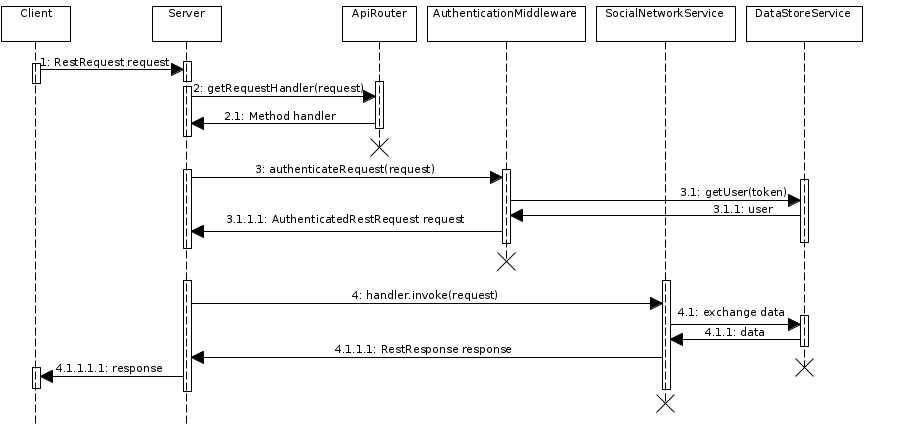
\includegraphics[width=\textwidth]{sequence2.png}

\subsection{La classe ServerConfig}
La classe \code{ServerConfig} rappresenta l'insieme delle impostazioni del server che, da specifica, devono poter essere regolate.
Il file di configurazione risulta quindi essere un file \textsc{json} contenente un'istanza serializzata di questa classe. Il vantaggio principale derivante dall'uso di questo approccio è
il riutilizzo delle componenti già esistenti all'interno del progetto: per leggere il file di configurazione basta, infatti, istanziare un \code{Serializer<ServerConfig>} e de-serializzare il contenuto del file
specificato.
\par Di default, il server utilizzerà il file \code{config.json} all'avvio, ma è possibile sovrascrivere questa impostazione eseguendo la classe \code{MainServer} con un argomento da linea di comando, per esempio
\code{java MainServer myconfig.json}.

\par Al fine di permettere di avviare il server con il minimo livello di configurazione manuale possibile, la classe \code{ServerConfig} è dotata di valori di default per ciascun \emph{setting}, che verranno utilizzati
se omessi nel file di configurazione scelto.

\par Il client, per semplicità, ha accesso a un riferimento a \code{ServerConfig} in maniera analoga al server: questo permette di reperire facilmente informazioni come l'indirizzo \textsc{ip} e la porta per avviare la connessione \textsc{tcp}.
Nell'ipotesi di un sistema realmente distribuito, dove client e server non risiedono sulla stessa macchina, si utilizzerebbe un sistema più sofisticato per il reperimento di tali dati, come per esempio l'accesso a un terzo servizio (se
il server fosse dotato di un nome di dominio, per esempio, basterebbe un lookup \textsc{dns}). Si noti che, seppure la maggior parte dei dati vengono letti dal client direttamente dall'istanza di \code{ServerConfig}, questo
non avviene per gli estremi del gruppo multicast, in quanto la specifica richiede che sia il server a comunicarli: essi vengono infatti inclusi nel corpo della risposta alle richieste di login.

\section{Il client \textsc{cli}}
All'avvio, il client reperisce utilizzando l'\textsc{rmi} \code{Registry} i servizi di registrazione utente e notifica per i follower, precedentemente esportati dal server.
Dopodiché, viene aperta una connessione \textsc{tcp} utilizzando un \code{SocketChannel} \textsc{nio}. Una volta stabilita la connessione al server, il client entra in un ciclo infinito
dove attende di leggere istruzioni da \code{stdin}. Ogni istruzione letta in input viene divisa in token in corrispondenza del carattere spazio: il primo token (o i primi due,
per le istruzioni composte da due parole) viene utilizzato per cercare corrispondenza con uno dei comandi supportati. Successivamente, vengono utilizzati tre metodi -- \code{getStringArgument},
\code{getIntArgument} e \code{getUUIDArgument}, a seconda del contesto -- per acquisire i parameteri del comando ricevuto, verificandone l'arietà e il tipo. Infine, se tutti i controlli hanno
esito positivo, viene chiamato il metodo handler corrispondente al comando con i parametri dati dall'utente.
\par Dopo aver effettuato il login, il client ottiene gli estremi (indirizzo \textsc{ip} e porta) per unirsi al gruppo multicast per le notifiche sugli aggiornamenti dei portafogli, inviatigli dal server
all'interno della risposta alla richiesta di autenticazione, e vi si connette in un thread separato. Il token di autenticazione altresì contenuto nella risposta viene salvato in una variabile locale e utilizzato per autenticare le richieste future.
Infine, una volta ottenuto il token, il client si registra via \textsc{rmi} callback al servizio di notifica per i follower. Il token viene passato come argomento al metodo per la registrazione, certificando così l'identità dell'utente.
\subsection{Gestione di una richiesta al server}
Gli handler del client implementano il seguente schema:
\begin{enumerate}
    \item Viene generata una \code{RestRequest} coi parametri (path, header e body) appropriati in base all'operazione
    \item Viene chiamato il metodo \code{receiveResponse}, che wrappa la richiesta in un \code{ByteBuffer} e la scrive sul socket che mantiene la connessione al server
    \item Viene letta la risposta. Se la risposta contiene un errore (codice \code{4xx} o \code{5xx}), viene sollevata una \code{ClientOperationFailedException}, altrimenti viene restituita la risposta allo handler chiamante
    \item All'interno dello handler, viene processato il contenuto della risposta. Il \emph{processing} effettuato dipende dalla semantica dell'operazione; nella maggior parte dei casi, viene istanziato un \code{Serializer} che ricostruisce un'entità (o un array di entità) e lo restituisce in uscita.
\end{enumerate}
La classe \code{ClientOperationFailedException} viene utilizzata per rappresentare il fallimento di un'interazione col server, dovuto nella maggior parte dei casi alla ricezione di una risposta \textsc{http} contenente un codice di errore.
Quando un'eccezione di questo tipo viene lanciata, possono esserle passati come parametro la richiesta e la risposta che costituiscono l'interazione fallita. Questi dati vengono utilizzati dal client per stampare il messaggio di errore appropriato (si veda la sezione \hyperref[sec:err_handling]{\emph{Gestione dei messaggi}}).

\subsection{Rendering dei dati}
La maggior parte delle operazioni svolte dal client si conclude con la stampa su \code{stdout} di dati ricevuti dal server. Per astrarre la logica di ricezione dei dati da quella
legata alla formattazione (o \emph{rendering}) degli stessi, si è utilizzata un'interfaccia parametrica dedicata: \code{IRenderer<E>}.

\par Le classi che implementano quest'interfaccia dispongono del metodo \code{render}, \emph{overloaded} in modo da poter essere utilizzato sia con singole istanze che con array. Il metodo
\code{render} si occupa, preso in input un oggetto del tipo assegnato dalla classe che implementa l'interfaccia, di formattarlo e restituire una stringa che rappresenta una versione \emph{pretty-printed} dell'oggetto.
\par Il client, all'atto della ricezione di dati dal server, istanzia un \code{Renderer} del tipo appropriato. Al termine dell'interazione, la stringa restituita dal renderer viene stampata su \code{stdout}.

\subsection{Gestione dei messaggi}
\label{sec:err_handling}
L'approccio scelto per la gestione dei messaggi (sia informativi che di errore) è di mantenerli in strutture dati separate dal resto del codice.
L'idea è quella di associare a ogni messaggio un codice mnemomico, e di accedere ai messaggi con un lookup nella struttura dedicata utilizzando il codice corrispondente.
\par L'utilizzo di questo metodo è motivato dall'obiettivo di disaccoppiare la logica del client dalla presentazione dei dati (non è buona pratica, in generale, avere \emph{magic strings} all'interno del codice). Inoltre,
come possibile estensione, si consideri cosa succederebbe se si volesse tradurre il client in più lingue. Disaccoppiando i messaggi dal codice dei vari metodi e impiegando un tool di traduzione, quale \href{https://docs.oracle.com/javase/8/docs/technotes/guides/intl/index.html}{\code{i18n}},
basterebbe modificare l'accesso alla struttura dati che contiene i messaggi testuali; diversamente, se le stringhe fossero \emph{hard-coded}, bisognerebbe intervenire sul codice modificandole \emph{una ad una}.
\par La maggior parte dei messaggi del client sono salvati all'interno della mappa \code{clientMessages}. Essa viene inizializzata e resa immutabile utilizzando la \emph{factory} \code{Collections.unmodifiableMap}.
\par Per avere un controllo più fine sui messaggi di errore, una seconda struttura viene impiegata: \\ \code{outcomeMessages}. Essa mappa nomi di path su mappe, che a loro volta mappano interi
(rappresentanti codici \textsc{http} di esito) su stringhe. L'idea è di fornire messaggi contestualizzati all'operazione e all'esito risultante.
La struttura in questione, popolata nello stesso modo della precedente, viene acceduta quando si verifica una \code{ClientOperationFailedException}, se essa non è già stata inizializzata con un messaggio: la \code{RestRequest} e \code{RestResponse} contenute nell'eccezione vengono utilizzate per il lookup nella mappa.

\section{Il client \textsc{gui}}
Il client \textsc{gui} è costituito da una web app realizzata utilizzando \textsc{html5} e \emph{vanilla} JavaScript.
È stato utilizzato il framework \href{https://tailwindcss.com/}{Tailwind \textsc{css}} per avere un set di classi di stile predefinite sopra le quali costruire il layout.
\par La motivazione dietro la realizzazione di un client web è di esemplificare il funzionamento del server anche con client eterogenei (in particolare, non scritti in Java), mostrando
che l'\textsc{api} esposta è \emph{compliant} con le specifiche \textsc{rest}/\textsc{rpc} e può essere consumata anche da browser.
\par Per avviare la web app, è sufficiente aprire con un browser il file \code{index.html} presente all'interno della cartella \code{guiClient}, nella root del progetto.

\subsection{Realizzazione}
La struttura della web app è quella di \emph{single-page application} (\textsc{spa}): tutte le funzionalità sono raggruppate all'interno di una singola pagina \textsc{html}, e l'utilizzo di JavaScript permette di mostrare programmaticamente
solo la parte di pagina inerente all'operazione che si sta svolgendo.
\par Le richieste \textsc{http} sono effettuate utilizzando la libreria \href{https://axios-http.com/docs/intro}{\textbf{Axios}}.
\par Il token di autenticazione ricevuto in fase di login viene salvato nei \emph{common headers} di Axios e automaticamente incluso nelle richieste effettuate dopo il login.
L'applicazione è dotata di un sistema \emph{ricordami}, che permette di aggiornare la pagina o chiudere e riaprire il browser rimanendo loggati. La funzionalità è implementata utilizzando
il \href{https://developer.mozilla.org/en-US/docs/Web/API/Window/localStorage?retiredLocale=it}{\code{localStorage}} di JavaScript: i dati vengono salvati nello storage del browser (in maniera simile ai cookie) e ripristinati
una volta riaperta la pagina web.

\subsection{Limitazioni}
Il client web implementa tutte e sole le funzionalità interagibili tramite l'\textsc{api} \textsc{rest}/\textsc{rpc} del server.
In altre parole, il sistema di registrazione utente, le notifiche per i follower e le notifiche multicast non sono presenti in questa versione del client.
\par Per ovviare all'impossibilità di registrarsi, si può registrare un utente utilizzando il client \textsc{cli} ed effettuare il login dal client web, oppure utilizzare l'utente
che viene \textbf{fornito di default} (incluso per permettere di testare agilmente la web app senza dover utilizzare prima il client \textsc{cli}): è sempre possibile, infatti, effettuare il login utilizzando lo username \code{admin} e la password \code{pass}.
\subsection{Alcuni screenshot dell'utilizzo della \textsc{gui}}
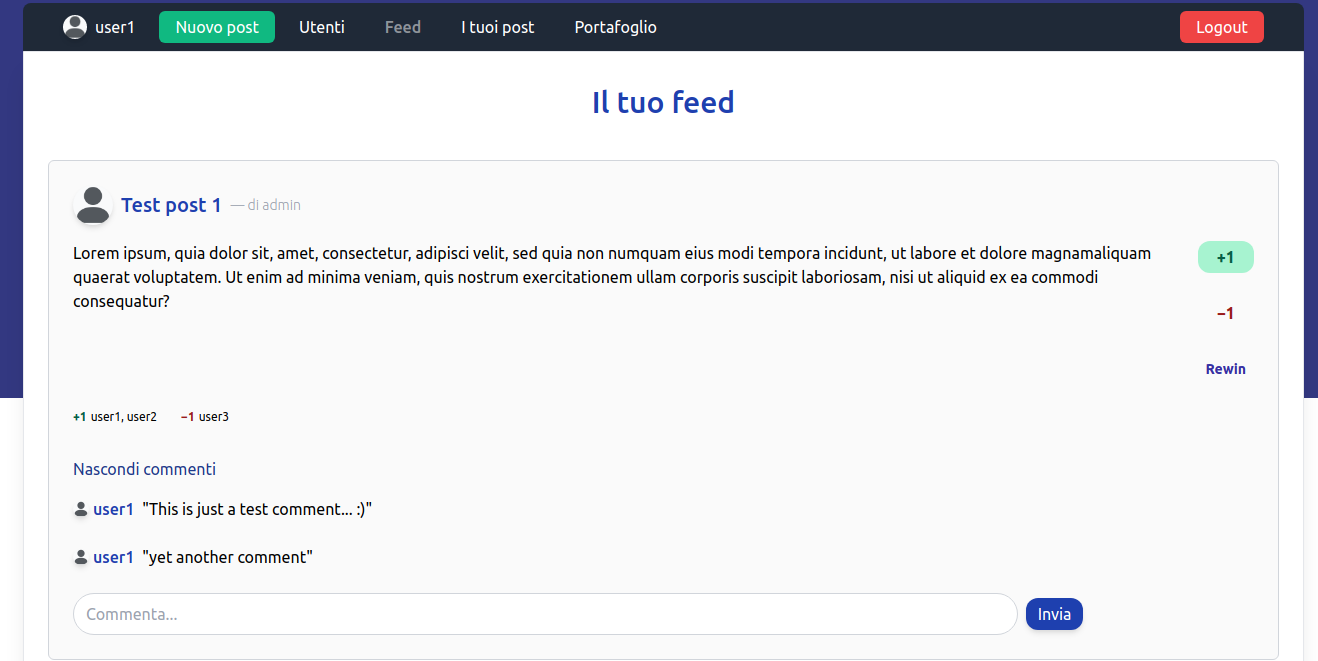
\includegraphics[width=\textwidth]{feed.png}\vspace*{0.5cm}
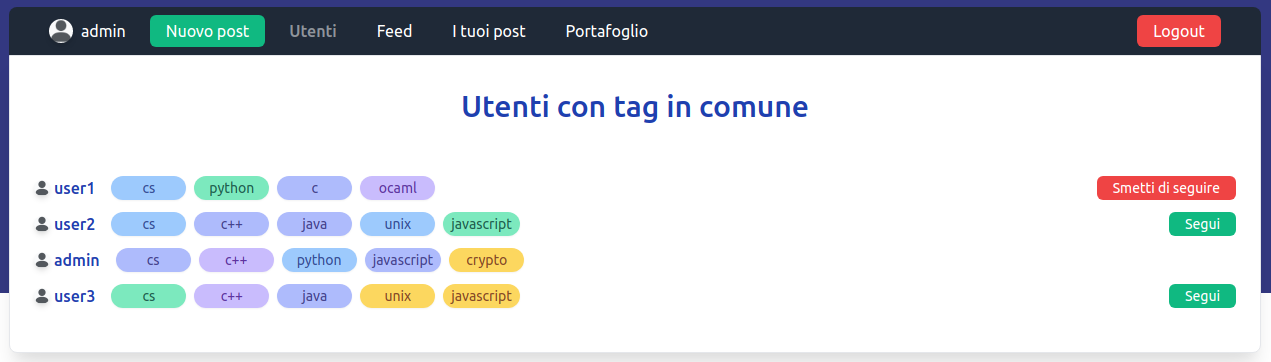
\includegraphics[width=\textwidth]{users.png}\vspace*{0.5cm}
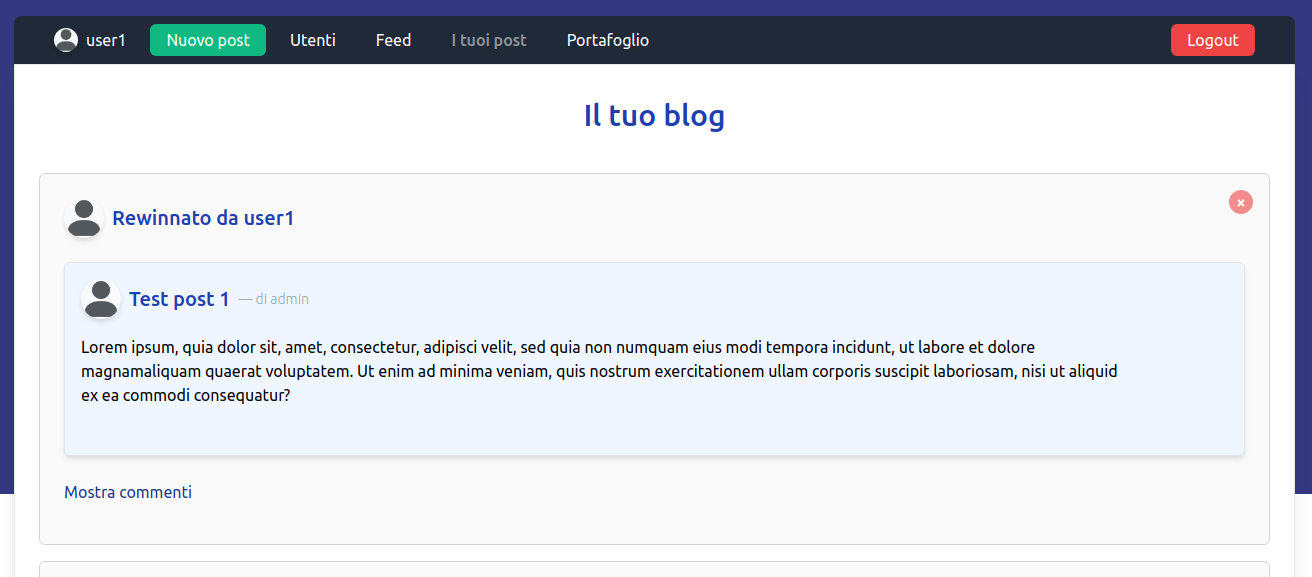
\includegraphics[width=\textwidth]{rewin.png}\newpage
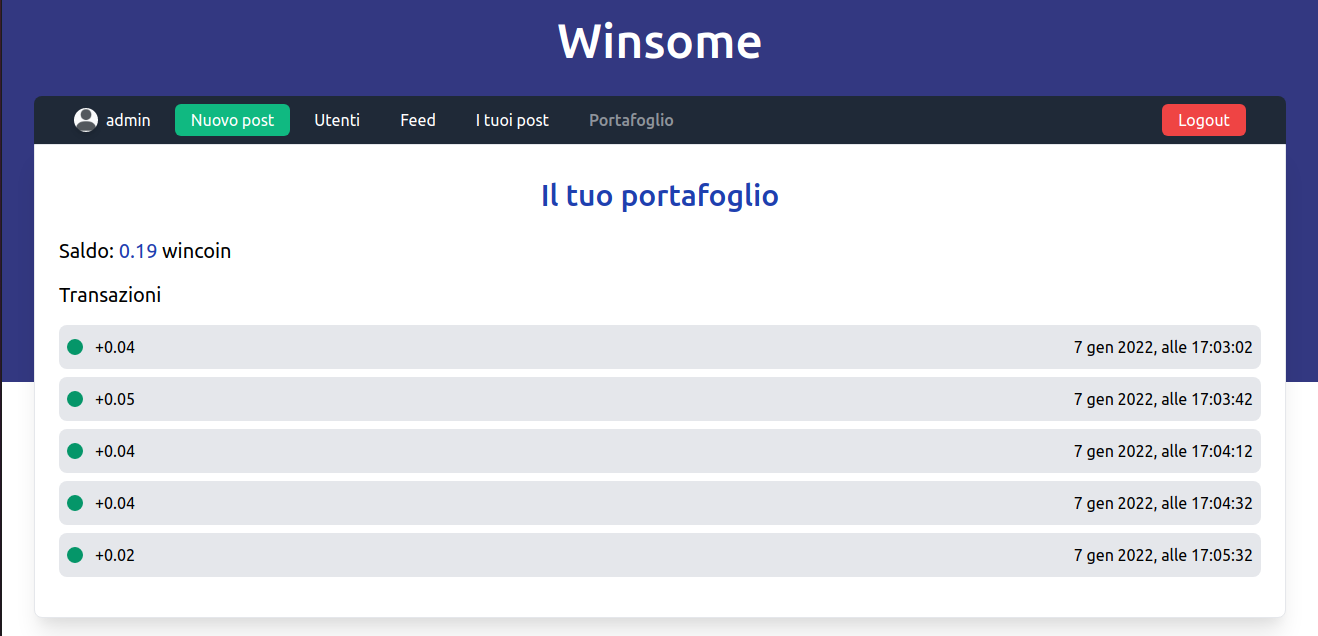
\includegraphics[width=\textwidth]{wallet.png}\vspace*{0.4cm}
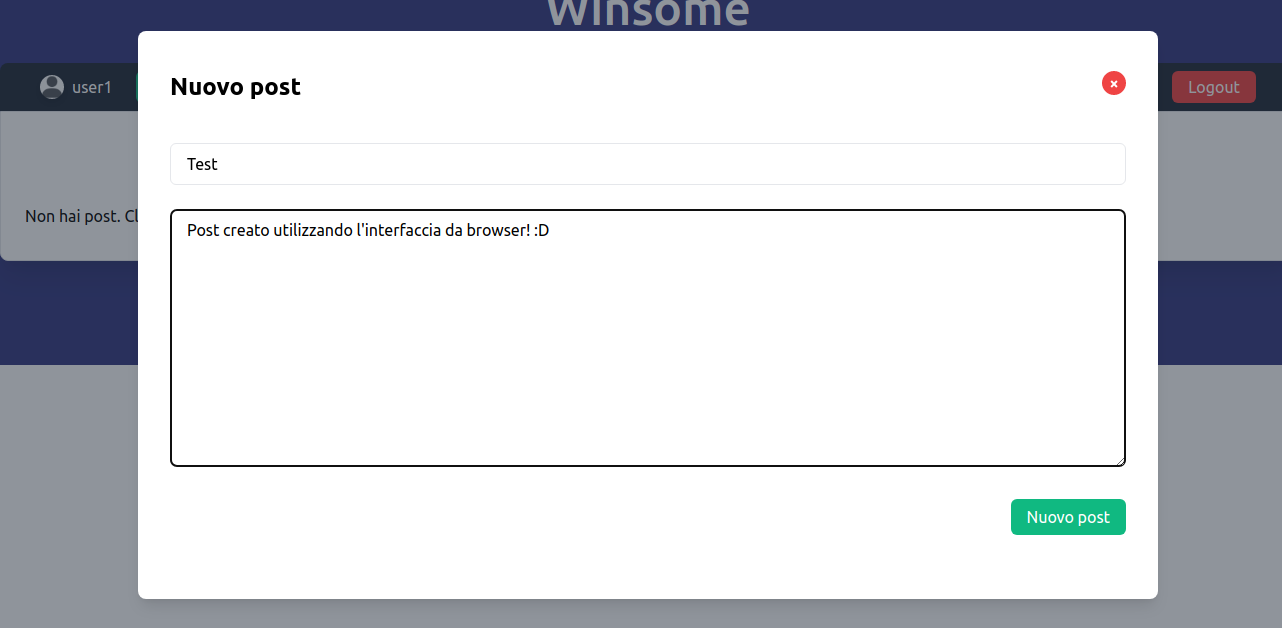
\includegraphics[width=\textwidth]{newpost.png}

\end{document}
